\chapter{Literature Review}

\textit{``Hunger roared up in him like a hopeless lust.\\ 
He walked the ship as though following a chart. Up. Down. Across. Back. Stem. Port. Stern. Starboard. The churning of the waves. \\
The ropes clanking on the masts. The blind of salt water. The wind ripping at the sails.''\\
\textemdash\ ``Star of the Sea'' by Joseph O'Connor}
\vspace{.2cm}

\section{A Brief Famine Outline}

The Irish lumper potato with its excellent ability to grow in poor and wet soils, was the predominant potato variety in pre-famine Ireland. It was introduced to U.K. around 1806 \citep{tucker2016potato}, and was rapidly replacing almost all other varieties in the recipes of the poor. Usually, on account of its intolerance of frost, the farmer sows in March or April, and the first early potatoes will be harvested in June, followed by the second early potatoes in July, and the third not later than October. With a 1.32 \% growth in lower class per year in Ireland from the centennial before 1841, in 1845 about 32\% of the arable land in Ireland was already under potato cultivation \citep{solar2015ireland}.

The first record of late blight on potatoes in Ireland is thought to be Dr Lindley's letter in September 16, 1845, with his concern words, he wrote: ``The potato murrain has unequivocally declared itself in Ireland, where will Ireland be in the event of a universal potato rot''? \citep{kelly1995great}. Things were getting worse in next year, a government documents collection book recorded that: ``the poor Irish lost their potatoes again'' (1 September, 1846),``Many, full many, must this winter leave their homes, and traverse the country in quest of work'' (15 September, 1846), ``to maintain Ireland's population, her agriculture must be greatly improved'' (31 October, 1846)


\section{Refuting some hypotheses}

This part I will refute some hypothesis of famine origin. Many people regard single factor as the root of the Great Famine.

\begin{figure}[h]
    \centering
    \caption{Food Structure}
    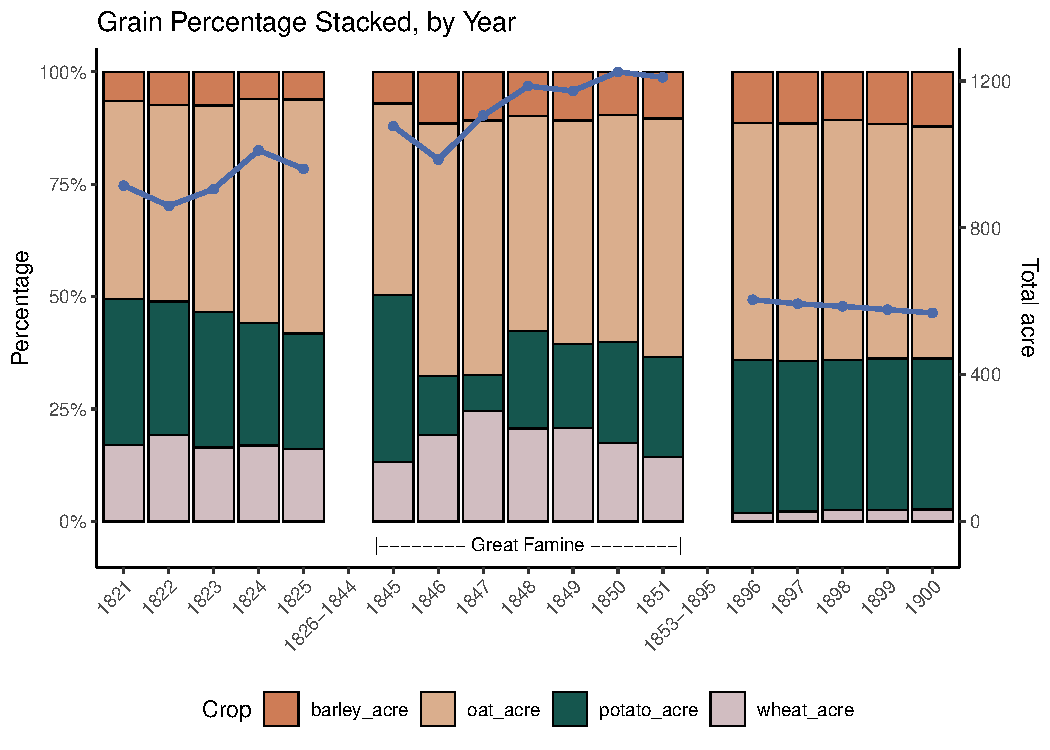
\includegraphics[width=.95\textwidth]{../03_outputs/food_structure.pdf}
\end{figure}

\subsection{Potato Blight}

In Nature journal,

1845 June Belgium, August France, August South of UK, September Ireland

\begin{figure}[h]
    \centering
    \caption{Food Structure}
    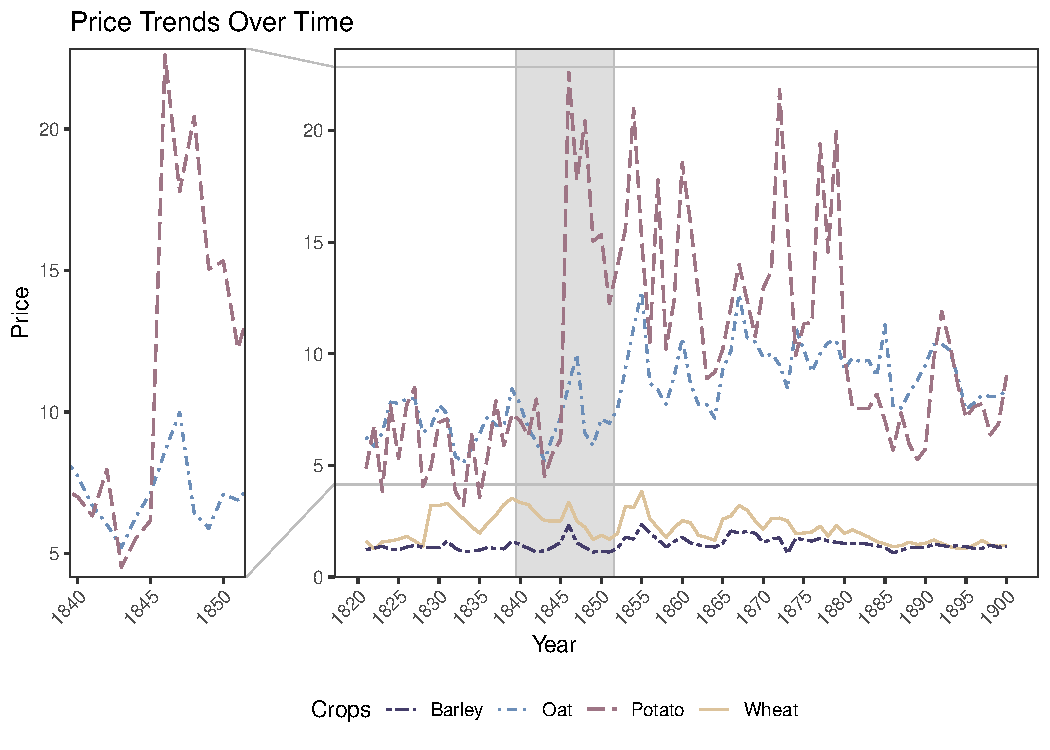
\includegraphics[width=.95\textwidth]{../03_outputs/grain_price.pdf}
\end{figure}



1. Blame potato blight as the only origin of famine

People believe potato blight was responsible for the Irish Great Famine. 

lumper potato

Blight became a semi-permanent fixture until the end of the century, when effective treatments were found \citep{o1994economic}.

2. Ireland have the bad land quality.

\section{Entitlement Approach}

I will operationalize entitlement approach into these 4 dimensions according to the book:

(1) trade-based entitlement: price, grain amount, 

(2) production-based entitlement: tax policy

(3) own-labour entitlement: wage, land own amount, poor law

(4) inheritance and transfer entitlement: none, hard to get data






